\documentclass[red]{beamer}
%\documentclass[handout]{beamer}

\usepackage{fixltx2e}
\usepackage{movie15}
\usepackage{hyperref}

%\usepackage[usenames,dvipsnames]{color}
%\usepackage[english]{babel}
\usepackage{tabularx}
\usepackage{soul}
\usepackage{xparse}
\usepackage{listings}


%%%%%%%%%%%%%%%
% Show a list of items "todo" or "done" 
% USAGE: 
% \begin{todolist} 
% 	\todo Something not finished
% 	\done Something finished
% \end{todolist} 
\newenvironment{todolist}{%
  \begin{list}{}{}% whatever you want the list to be
  \let\olditem\item
  \renewcommand\item{\olditem \textcolor{red}{(TODO)}: }
  \newcommand\todo{\olditem \textcolor{red}{(TODO)}: }
   \newcommand\done{\olditem \textcolor{ForestGreen}{(DONE)}: }
}{%
  \end{list}
} 
%%%%%%%%%%%%%%%



%%%%%%%%%%%%%%%
% Show a Author's Note
% USAGE: 
% \authnote[Optional footnote message to further clarify note]{The note to your readers}
\DeclareDocumentCommand \authnote { o m }
{%
\IfNoValueTF {#1}
{\textcolor{blue}{Author's Note: \uline{#2}}} 
{\textcolor{blue}{Author's Note: \uline{#2}}\footnote{Comment: #1}}%
}
%%%%%%%%%%%%%%%



%%%%%%%%%%%%%%%
% Strike out text that doesn't belong in the paper
% USAGE: 
% \strike[Optional footnote to state why it doesnt belong]{Text to strike out}
\DeclareDocumentCommand \strike { o m }
{%
\IfNoValueTF {#1}
{\textcolor{red}{\sout{#2}}} 
{\textcolor{red}{\sout{#2}}\footnote{Comment: #1}}%
}
%%%%%%%%%%%%%%%

\definecolor{light-gray}{gray}{0.95}

\newcommand{\cbox}[3]{
\ \\
\fcolorbox{#1}{#2}{
\parbox{\textwidth}{
#3
}
}
}

% Setup an environment similar to verbatim but which will highlight any bash commands we have
\lstnewenvironment{unixcmds}[0]
{
%\lstset{language=bash,frame=shadowbox,rulesepcolor=\color{blue}}
\lstset{ %
language=sh,		% Language
basicstyle=\ttfamily,
backgroundcolor=\color{light-gray}, 
rulecolor=\color{blue},
%frame=tb, 
columns=fullflexible,
%framexrightmargin=-.2\textwidth,
linewidth=0.8\textwidth,
breaklines=true,
%prebreak=/, 
  prebreak = \raisebox{0ex}[0ex][0ex]{\ensuremath{\hookleftarrow}},
%basicstyle=\footnotesize,       % the size of the fonts that are used for the code
%numbers=left,                   % where to put the line-numbers
%numberstyle=\footnotesize,      % the size of the fonts that are used for the line-numbers
%stepnumber=2,                   % the step between two line-numbers. If it's 1 each line 
                                % will be numbered
%numbersep=5pt,                  % how far the line-numbers are from the code
showspaces=false,               % show spaces adding particular underscores
showstringspaces=false,         % underline spaces within strings
showtabs=false,                 % show tabs within strings adding particular underscores
frame=single,	                % adds a frame around the code
tabsize=2,	                % sets default tabsize to 2 spaces
captionpos=b,                   % sets the caption-position to bottom
breakatwhitespace=false,        % sets if automatic breaks should only happen at whitespace
}
} { }

% Setup an environment similar to verbatim but which will highlight c++ syntax
\lstnewenvironment{cppcode}[1]
{
%\lstset{language=bash,frame=shadowbox,rulesepcolor=\color{blue}}
\lstset{ %
	backgroundcolor=\color{light-gray},
	rulecolor=\color[rgb]{0.133,0.545,0.133},
	tabsize=4,
	language=[GNU]C++,
%	basicstyle=\ttfamily,
        basicstyle=\scriptsize,
        upquote=true,
        aboveskip={1.5\baselineskip},
        %columns=fullflexible,
        %framexrightmargin=-.1\textwidth,
       %framexleftmargin=6mm,
        showstringspaces=false,
        extendedchars=true,
        breaklines=true,
        prebreak = \raisebox{0ex}[0ex][0ex]{\ensuremath{\hookleftarrow}},
        frame=single,
        showtabs=false,
        tabsize=4,
        showspaces=false,
        showstringspaces=false,
        numbers=left,                   % where to put the line-numbers
        numbers=none,                   % where to put the line-numbers
	numberstyle=\footnotesize,      % the size of the fonts that are used for the line-numbers
	stepnumber=4,                   % the step between two line-numbers. If it's 1 each line 
                                % will be numbered
	firstnumber=#1,
         numbersep=5pt,                  % how far the line-numbers are from the code
        identifierstyle=\ttfamily,
        keywordstyle=\color[rgb]{0,0,1},
        commentstyle=\color[rgb]{0.133,0.545,0.133},
        stringstyle=\color[rgb]{0.627,0.126,0.941},
}
} { }

% Setup an environment similar to verbatim but which will highlight any bash commands we have
\lstnewenvironment{mcode}[1]
{
\lstset{ %
	backgroundcolor=\color{light-gray}, 
	rulecolor=\color[rgb]{0.133,0.545,0.133},
	tabsize=4,
	language=Matlab,
%	basicstyle=\ttfamily,
        basicstyle=\scriptsize,
        upquote=true,
        aboveskip={1.5\baselineskip},
        columns=fullflexible,
        %framexrightmargin=-.1\textwidth,
       %framexleftmargin=6mm,
        showstringspaces=false,
        extendedchars=true,
        breaklines=true,
        prebreak = \raisebox{0ex}[0ex][0ex]{\ensuremath{\hookleftarrow}},
        frame=single,
        showtabs=false,
        showspaces=false,
        showstringspaces=false,
        numbers=left,                   % where to put the line-numbers
	numberstyle=\footnotesize,      % the size of the fonts that are used for the line-numbers
	stepnumber=4,                   % the step between two line-numbers. If it's 1 each line 
                                % will be numbered
	firstnumber=#1,
         numbersep=5pt,                  % how far the line-numbers are from the code
        identifierstyle=\ttfamily,
        keywordstyle=\color[rgb]{0,0,1},
        commentstyle=\color[rgb]{0.133,0.545,0.133},
        stringstyle=\color[rgb]{0.627,0.126,0.941},
}
} { }

\newcommand{\inputmcode}[1]{%
\lstset{ %
	backgroundcolor=\color{light-gray},  %
	rulecolor=\color[rgb]{0.133,0.545,0.133}, %
	tabsize=4, %
	language=Matlab, %
%	basicstyle=\ttfamily,
        basicstyle=\scriptsize, %
        %        upquote=true,
        aboveskip={1.5\baselineskip}, %
        columns=fullflexible, %
        %framexrightmargin=-.1\textwidth,
       %framexleftmargin=6mm,
        showstringspaces=false, %
        extendedchars=true, %
        breaklines=true, %
        prebreak = \raisebox{0ex}[0ex][0ex]{\ensuremath{\hookleftarrow}}, %
        frame=single, %
        showtabs=false, %
        showspaces=false, %
        showstringspaces=false,%
        numbers=left,                   % where to put the line-numbers
	numberstyle=\footnotesize,      % the size of the fonts that are used for the line-numbers
	stepnumber=4,                   % the step between two line-numbers. If it's 1 each line 
                                % will be numbered
         numbersep=5pt,                  % how far the line-numbers are from the code
        identifierstyle=\ttfamily, %
        keywordstyle=\color[rgb]{0,0,1}, %
        commentstyle=\color[rgb]{0.133,0.545,0.133}, %
        stringstyle=\color[rgb]{0.627,0.126,0.941} %
}
\lstinputlisting{#1}%
}

%\lstset{ %
%	backgroundcolor=\color{light-gray}, 
%	rulecolor=\color[rgb]{0.133,0.545,0.133},
%	tabsize=4,
%	language=Matlab,
%%	basicstyle=\ttfamily,
%        basicstyle=\scriptsize,
%        upquote=true,
%        aboveskip={1.5\baselineskip},
%        columns=fullflexible,
%        %framexrightmargin=-.1\textwidth,
%       %framexleftmargin=6mm,
%        showstringspaces=false,
%        extendedchars=true,
%        breaklines=true,
%        prebreak = \raisebox{0ex}[0ex][0ex]{\ensuremath{\hookleftarrow}},
%        frame=single,
%        showtabs=false,
%        showspaces=false,
%        showstringspaces=false,
%        numbers=left,                   % where to put the line-numbers
%	numberstyle=\footnotesize,      % the size of the fonts that are used for the line-numbers
%	stepnumber=4,                   % the step between two line-numbers. If it's 1 each line 
%                                % will be numbered
%	firstnumber=#1,
%         numbersep=5pt,                  % how far the line-numbers are from the code
%        identifierstyle=\ttfamily,
%        keywordstyle=\color[rgb]{0,0,1},
%        commentstyle=\color[rgb]{0.133,0.545,0.133},
%        stringstyle=\color[rgb]{0.627,0.126,0.941},
%}


\newcommand{\Laplacian}[1]{\nabla^2 #1}

% set of all nodes received and contained on GPU
\newcommand{\setAllNodes}[0]{\mathcal{G}}
% set of stencil centers on GPU
\newcommand{\setCenters}[0]{\mathcal{Q}}
% set of stencil centers with nodes in \setDepend
\newcommand{\setBoundary}[0]{\mathcal{B}}
% set of nodes received by other GPUs
\newcommand{\setDepend}[0]{\mathcal{R}}
% set of nodes sent to other GPUs
\newcommand{\setProvide}[0]{\mathcal{O}}


\newcommand{\toprule}[0]{\hline}
\newcommand{\midrule}[0]{\hline\hline}
\newcommand{\bottomrule}[0]{\hline}

\newcolumntype{C}{>{\centering\arraybackslash}b{1in}}
\newcolumntype{L}{>{\flushleft\arraybackslash}b{1.5in}}
\newcolumntype{R}{>{\flushright\arraybackslash}b{1.5in}}
\newcolumntype{D}{>{\flushright\arraybackslash}b{2.0in}}
\newcolumntype{E}{>{\flushright\arraybackslash}b{1.0in}}

\DeclareSymbolFont{AMSb}{U}{msb}{m}{n}
\DeclareMathSymbol{\N}{\mathbin}{AMSb}{"4E}
\DeclareMathSymbol{\Z}{\mathbin}{AMSb}{"5A}
\DeclareMathSymbol{\R}{\mathbin}{AMSb}{"52}
\DeclareMathSymbol{\Q}{\mathbin}{AMSb}{"51}
\DeclareMathSymbol{\PP}{\mathbin}{AMSb}{"50}
\DeclareMathSymbol{\I}{\mathbin}{AMSb}{"49}
\DeclareMathSymbol{\C}{\mathbin}{AMSb}{"43}

%%%%%% VECTOR NORM: %%%%%%%
\newcommand{\vectornorm}[1]{\left|\left|#1\right|\right|}
%\renewcommand{\vec}[1]{ \textbf{#1} }
%%%%%%%%%%%%%%%%%%%%%%

%%%%%%% THM, COR, DEF %%%%%%%
%\newtheorem{theorem}{Theorem}[section]
%\newtheorem{lemma}[theorem]{Lemma}
%\newtheorem{proposition}[theorem]{Proposition}
%\newtheorem{corollary}[theorem]{Corollary}
%\newenvironment{proof}[1][Proof]{\begin{trivlist}
%\item[\hskip \labelsep {\bfseries #1}]}{\end{trivlist}}
%\newenvironment{definition}[1][Definition]{\begin{trivlist}
%\item[\hskip \labelsep {\bfseries #1}]}{\end{trivlist}}
%\newenvironment{example}[1][Example]{\begin{trivlist}
%\item[\hskip \labelsep {\bfseries #1}]}{\end{trivlist}}
%\newenvironment{remark}[1][Remark]{\begin{trivlist}
%\item[\hskip \labelsep {\bfseries #1}]}{\end{trivlist}}
%\newcommand{\qed}{\nobreak \ifvmode \relax \else
%      \ifdim\lastskip<1.5em \hskip-\lastskip
%      \hskip1.5em plus0em minus0.5em \fi \nobreak
%      \vrule height0.75em width0.5em depth0.25em\fi}
%%%%%%%%%%%%%%%%%%%%%%

%
%\usepackage[algochapter]{algorithm2e}
%\usepackage[usenames]{color}
% colors to show the corrections
\newcommand{\red}[1]{\textbf{\textcolor{red}{#1}}}
\newcommand{\blue}[1]{\textbf{\textcolor{blue}{#1}}}
\newcommand{\cyan}[1]{\textbf{\textcolor{cyan}{#1}}}
\newcommand{\green}[1]{\textbf{\textcolor{green}{#1}}}
\newcommand{\magenta}[1]{\textbf{\textcolor{magenta}{#1}}}
\newcommand{\orange}[1]{\textbf{\textcolor{orange}{#1}}}
%%%%%%%%%% DK DK
% comments between authors
\newcommand{\toall}[1]{\textbf{\green{@@@ All: #1 @@@}}}
\newcommand{\toevan}[1]{\textbf{\red{*** Evan: #1 ***}}}
\newcommand{\toe}[1]{\textbf{\red{*** Evan: #1 ***}}}

\newcommand{\tog}[1]{\textbf{\blue{*** Gordon: #1 ***}}}
\newcommand{\toi}[1]{\textbf{\magenta{*** Ian: #1 ***}}}
\newcommand{\togordon}[1]{\textbf{\blue{*** Gordon: #1 ***}}}
\newcommand{\gee}[1]{{\bf{\blue{{\em #1}}}}}
\newcommand{\old}[1]{}
\newcommand{\del}[1]{***#1*** }



% \DeclareMathOperator{\Sample}{Sample}
%\let\vaccent=\v % rename builtin command \v{} to \vaccent{}
%\renewcommand{\vec}[1]{\ensuremath{\mathbf{#1}}} % for vectors
\newcommand{\gv}[1]{\ensuremath{\mbox{\boldmath$ #1 $}}} 
% for vectors of Greek letters
\newcommand{\uv}[1]{\ensuremath{\mathbf{\hat{#1}}}} % for unit vector
\newcommand{\abs}[1]{\left| #1 \right|} % for absolute value
\newcommand{\avg}[1]{\left< #1 \right>} % for average
\let\underdot=\d % rename builtin command \d{} to \underdot{}
\renewcommand{\d}[2]{\frac{d #1}{d #2}} % for derivatives
\newcommand{\dd}[2]{\frac{d^2 #1}{d #2^2}} % for double derivatives
\newcommand{\pd}[2]{\frac{\partial #1}{\partial #2}} 
% for partial derivatives
\newcommand{\pdd}[2]{\frac{\partial^2 #1}{\partial #2^2}} 
\newcommand{\pdda}[3]{\frac{\partial^2 #1}{\partial #2 \partial #3}} 
% for double partial derivatives
\newcommand{\pdc}[3]{\left( \frac{\partial #1}{\partial #2}
 \right)_{#3}} % for thermodynamic partial derivatives
\newcommand{\ket}[1]{\left| #1 \right>} % for Dirac bras
\newcommand{\bra}[1]{\left< #1 \right|} % for Dirac kets
\newcommand{\braket}[2]{\left< #1 \vphantom{#2} \right|
 \left. #2 \vphantom{#1} \right>} % for Dirac brackets
\newcommand{\matrixel}[3]{\left< #1 \vphantom{#2#3} \right|
 #2 \left| #3 \vphantom{#1#2} \right>} % for Dirac matrix elements
\newcommand{\grad}[1]{\gv{\nabla} #1} % for gradient
\let\divsymb=\div % rename builtin command \div to \divsymb
\renewcommand{\div}[1]{\gv{\nabla} \cdot #1} % for divergence
\newcommand{\curl}[1]{\gv{\nabla} \times #1} % for curl
\let\baraccent=\= % rename builtin command \= to \baraccent
\renewcommand{\=}[1]{\stackrel{#1}{=}} % for putting numbers above =
\newcommand{\diffop}[1]{\mathcal{L}#1}
\newcommand{\boundop}[1]{\mathcal{B}#1}
\newcommand{\rvec}[0]{{\bf r}}

\newcommand{\Interior}[0]{\Omega}
\newcommand{\Boundary}[0]{\partial \Omega}

\newcommand{\on}[1]{\hskip1.5em \textrm{ on } #1}

\newcommand{\gemm}{\texttt{GEMM}}
\newcommand{\trmm}{\texttt{TRMM}}
\newcommand{\gesvd}{\texttt{GESVD}}
\newcommand{\geqrf}{\texttt{GEQRF}}


\newcommand{\minitab}[2][l]{\begin{tabular}{#1}#2\end{tabular}}
\newcommand{\comm}[1]{\textcolor{red}{\textit{#1}}}

\newcommand{\nfrac}[2]{
\nicefrac{#1}{#2}
%\frac{#1}{#2}
}

%\input{../misc_mac.tex}

%\usetheme{MyTheme} 
%\usetheme{Berkeley}
\usetheme{Copenhagen}

% title
\title[Flocking Implementation for the Blender Game Engine]{Flocking Implementation for the Blender Game Engine}
\author{Myrna I. Merced Serrano}
\institute{\textbf{Adviser:} Dr. Gordon Erlebacher}
\date{June 24\textsuperscript{th}, 2011}

\setcounter{tocdepth}{1}

\begin{document}

%--------------------------------------------
% title 
%--------------------------------------------
\begin{frame}
	\titlepage
\end{frame}

%--------------------------------------------
% table of contents
%--------------------------------------------
\begin{frame}
	\tableofcontents
\end{frame}

%--------------------------------------------
% motivation - intro
%--------------------------------------------
\section{Motivation}

%--------------------------------------------
% educational games
%--------------------------------------------
\subsection{Educational Games}
\begin{frame}{Motivation}
	\begin{itemize}
		\pause \item Develop tools for educational games.
		\pause \item Address the poor performance in the basic classes of students.
		\pause \item Incorporate general tools such as flocking into public domain game engines.
	\end{itemize}	
\end{frame}

%--------------------------------------------
% related work
%--------------------------------------------
\subsection{Background and Related Work}

% flocking
\begin{frame}{Flocking}
	\begin{itemize}
		\pause \item \textit{Flocking} is a nature-inspired behavior, mostly seen in animals.
		\pause \item Collective motion of large group of entities, that exhibits interesting behavior as a whole.
	\end{itemize}
\end{frame}

\begin{frame}{Flocking}
	\begin{figure}[htbp]
	\begin{center}
	\includegraphics[scale=2.25]{figures/flock.pdf} 
	\end{center}
	\caption{Flocking behavior: Flock of birds}
	\label{default}
	\end{figure}

\end{frame}

\begin{frame}{Flocking}
	\begin{figure}[htbp]
	\begin{center}
	\includegraphics[scale=.55]{figures/school.pdf} 
	\end{center}
	\caption{Flocking behavior: Schooling}
	\label{default}
	\end{figure}

\end{frame}

\begin{frame}{Flocking}
	\begin{figure}[htbp]
	\begin{center}
	\includegraphics[scale=0.4]{figures/herd.pdf} 
	\end{center}
	\caption{Flocking behavior: Herd of quadrupeds}
	\label{default}
	\end{figure}

\end{frame}

\begin{frame}{Flocking}
	\begin{figure}[htbp]
	\begin{center}
	\includegraphics[scale=0.5]{figures/swarm.pdf}
	\end{center}
	\caption{Flocking behavior: Swarms of insects}
	\label{default}
	\end{figure}

\end{frame}


\begin{frame}{Flocking}
	\begin{itemize}
		\pause \item Inspired by the flocking behavior of birds Craig Reynolds developed a behavioral model that simulated the self-organization of \textit{boids}.
		\pause \item \textit{Boids} are the entities of a flock.
		\pause \item Craig Reynolds is the pioneer of flocking, his most recognized paper: \textit{Flocks, herds, and school: A Distributed Behavioral Model} revolutionized the field of flocking.
	\end{itemize}
\end{frame}

% craig
\begin{frame}{Original Boids Model by Craig Reynolds}
	\pause The set of rules, also called \textit{Boids Model}, consist of:
	
	\begin{columns}[b]
		\pause
		\begin{column}{4cm}
			\begin{figure}[htbp]
			\begin{center}
			\includegraphics[scale=0.1]{../figures/sep_Craig.pdf}
			\caption{Collision Avoidance}
			\end{center}
			\end{figure}
		\end{column}
		\pause
		\begin{column}{4cm}
			\begin{figure}[htbp]
			\begin{center}
			\includegraphics[scale=0.1]{../figures/align_Craig.pdf}
			\caption{Velocity Matching}
			\end{center}
			\end{figure}
		\end{column}
		\pause
		\begin{column}{4cm}
			\begin{figure}[htbp]
			\begin{center}
			\includegraphics[scale=0.1]{../figures/coh_Craig.pdf}
			\caption{Flock Centering}
			\end{center}
			\end{figure}
		\end{column}
	\end{columns}		
\end{frame}


% other rules
\begin{frame}{Previous Flocking Work}
	\begin{columns}[b]
		\begin{column}{6cm}
			\pause
			\begin{figure}[htbp]
			\begin{center}
			\includegraphics[scale=0.2]{../figures/seek.pdf}
			\caption{Seek and Pursuit}
			\end{center}
			\end{figure} 
		\end{column}
	
		\begin{column}{6cm}
			\pause
			\begin{figure}[htbp]
			\begin{center}
			\includegraphics[scale=0.2]{../figures/avoid.pdf}
			\caption{Flee and Evasion}
			\end{center}
			\end{figure}
		\end{column}
	\end{columns}
\end{frame}
		
\begin{frame}{Previous Flocking Work}
	\begin{columns}[b]
		\begin{column}{6cm}
			\pause
			\begin{figure}[htbp]
			\begin{center}
			\includegraphics[scale=0.2]{../figures/obstacle.pdf}
			\caption{Obstacle Avoidance}
			\end{center}
			\end{figure} 
		\end{column}
	
		\begin{column}{6cm}
			\pause
			\begin{figure}[htbp]
			\begin{center}
			\includegraphics[scale=0.2]{../figures/pathFollowing.pdf}
			\caption{Path Following}
			\end{center}
			\end{figure}
		\end{column}
	\end{columns}
\end{frame}		
			
			
% applications
\begin{frame}{Applications}
	\pause Prey and predator simulations
	\begin{figure}[htbp]
	\begin{center}
	\includegraphics[scale=1]{figures/predatorPrey.pdf}
	\caption{Prey flock escaping from predator from \textit{Predator�s attack-induced phase-like transition in prey flock}}
	\end{center}
	\end{figure}	
\end{frame}

\begin{frame}{Applications}		
 	Crowding simulations
	\begin{figure}[htbp]
	\begin{center}
	\includegraphics[scale=0.4]{figures/crowds.pdf}
	\caption{10,000 schooling fish from \textit{Big Fast Crowds on PS3}}
	\end{center}
	\end{figure}
\end{frame}

\begin{frame}{Applications}	
	Robotics
	\begin{figure}[htbp]
	\begin{center}
	\includegraphics[scale=0.2]{figures/robots.pdf}
	\caption{Obstacle avoidance of robots from \textit{A Decentralized and Adaptive Flocking Algorithm for Autonomous Mobile Robots}}
	\end{center}
	\end{figure}	
\end{frame}

\begin{frame}{Applications}
	Document clustering
	\begin{figure}[htbp]
	\begin{center}
	\includegraphics[scale=3.5]{figures/documents.pdf}
	\caption{Flocking clustering on 800 two-dimensional objects from \textit{A flocking based algorithm for document clustering analysis}}
	\end{center}
	\end{figure}
\end{frame}

% GPU computing
\begin{frame}{GPU Computing}
	\begin{itemize}
		\pause \item Graphical processing units or \textit{GPUs} are numeric computing engines used to perform a massive number of floating-point calculations in parallel.
		\pause \item \textit{GPU computing}, also know as \textit{GPGPU} is a field of study that develops the use of GPUs for general computing.
		\pause \item GPU computing is often considered an heterogeneous system, a mixture of GPUs and CPUs used together to process one or more tasks.
		\pause \item GPUs have different architecture than the CPUs therefore, they need to be programmed in a special manner.
	\end{itemize}
\end{frame}

% flocking using the GPU
\begin{frame}{Flocking Using the GPU}
	\begin{itemize}
		\pause \item Flocking algorithms are parallelizable algorithms because the same operations are computed for all boids in the flock.
		\pause \item GPUs can be used to implement flocking algorithms and allow flocks with tens or hundreds of thousands of boids.
	\end{itemize}
\end{frame}

%--------------------------------------------
% aim
%--------------------------------------------
\subsection{Aim}
\begin{frame}{Aim}
	\begin{itemize}
		\pause \item To develop a flocking implementation that can be used in the Blender Game Engine.
	\end{itemize}
\end{frame}

%--------------------------------------------
% flocking algorithm
%--------------------------------------------
\section{Algorithm}

\begin{frame}{Flocking}
	\begin{itemize}
		\pause \item \textit{Flocking} is used to simulate social behavior between entities by following a simple set of rules.
		\pause \item The three main rules, also called \textit{steering behaviors} are:
			\begin{itemize}
				\pause \item Separation
				\pause \item Alignment
				\pause \item Cohesion
			\end{itemize}
		\pause \item Each rule is associated to a velocity vector and a scalar weight.
	\end{itemize}
\end{frame}

%--------------------------------------------
% 3 behaviors
%--------------------------------------------
\subsection{Three Main Steering Behaviors}

% separation
\begin{frame}{Separation}
	% equation: separation 
	\begin{equation}
	\label{separationEquation}
	Separation =\frac{1}{M} \sum_{n=1}^{M} \frac{p_i - p_n}{d(p_i,p_n)}
	\end{equation}
	
	% figure: separation
	\begin{figure}[htbp]
	\begin{center}
	\includegraphics[scale=0.25]{../figures/separation.pdf}
	%\caption{Separation steering behavior}
	\label{separation}
	\end{center}
	\end{figure}
\end{frame}

% alignment
\begin{frame}{Alignment}
	% equation: alignment
	\begin{equation}
	\label{alignmentEquation}
	Alignment = \left[  \frac{1}{N} \sum_{n=1}^{N} v_n \right ] - v_i
	\end{equation}
	
	% figure: alignment
	\begin{figure}[htbp]
	\begin{center}
	\includegraphics[scale=0.25]{../figures/alignment.pdf}
	%\caption{Alignment steering behavior}
	\label{alignment}
	\end{center}
	\end{figure}
\end{frame}

% cohesion
\begin{frame}{Cohesion}
	% equation: cohesion
	\begin{equation}
	\label{cohesionEquation}
	Cohesion = \left[  \frac{1}{N} \sum_{n=1}^{N} p_n \right ] - p_i
	\end{equation}
	
	% figure: cohesion
	\begin{figure}[htbp]
	\begin{center}
	\includegraphics[scale=0.25]{../figures/cohesion.pdf}
	%\caption{Cohesion steering behavior}
	\label{cohesion}
	\end{center}
	\end{figure}
\end{frame}

%--------------------------------------------
% other behaviors
%--------------------------------------------
\subsection{Other Steering Behaviors}

% goal 
\begin{frame}{Goal}
	% goal equation
	\begin{equation}
	\label{goalEquation}
	Goal = \left(\frac{p_t - p_i}{d(p_t,p_i)} * max_{speed}\right) - v_i
	\end{equation}
	
	% figure: seek and flee
	\begin{figure}[htbp]
	\begin{center}
	\includegraphics[scale=0.45]{../figures/goal.pdf}
	%\caption{Goal steering behavior}
	\label{seekANDflee}
	\end{center}
	\end{figure}
\end{frame}

% avoid
\begin{frame}{Avoidance}
	\begin{equation}
	\label{avoidEquation}
	Avoidance = -\left(\frac{p_t - p_i}{d(p_t,p_i)} * max_{speed}\right) - v_i
	\end{equation}

	% figure: seek and flee
	\begin{figure}[htbp]
	\begin{center}
	\includegraphics[scale=0.45]{../figures/avoidance.pdf}
	%\caption{Avoidance steering behavior}
	\label{seekANDflee}
	\end{center}
	\end{figure}
\end{frame}
% avoid equation
	
% combine
\begin{frame}{Final Velocity}
	\pause The final velocity of the boids is calculated by doing a linear combination of the steering behaviors.
	 
	\begin{equation}
	vel^{k+1} = vel^{k} + \sum_{rule_r} w_{rule_r} {rule_r}
	\end{equation}
	
	where ${rule}_r$ is the resulting velocity of each steering behavior and $w_{rule_r}$ is the respective scalar weight for that rule. 
	 
\end{frame}

%--------------------------------------------
% algorithm
%--------------------------------------------
\subsection{Flocking Algorithm}

% rules
\begin{frame}{Algorithm to compute the rules}
	\alert<1>{$for$ each boid $i$ $do$}	 \\
	\alert<2>{~~$for$ each neighbor $j$ of boid $i$ $do$}			\\
	\alert<3>{~~~~$if$ d($pos_i$, $pos_j$) $<=$ searching radius $then$}	\\
	\alert<4>{~~~~~~$if$ $w_{rule_r}$ $>$ 0 $then$}					\\
	\alert<4>{~~~~~~~~~~Compute $rule_r$}  \\
	\alert<4>{~~~~~~end $if$} \\
	\alert<5>{~~~~~~$Comment: Compute ~all ~the ~other ~rules. $} \\
	\alert<3>{~~~~end $if$} \\
	\alert<2>{~~end $for$} \\
	\alert<1>{end $for$}
\end{frame}

% integration
\begin{frame}{Combine and Integrate}
 	\alert<1>{$vel_{rule_r}$ = $rule_r$ $w_{rule_r}$}			\\
	\alert<2>{$vel_i^{k+1} = vel_i^{k} + \sum_{rule_r} vel_{rule_r}$} 	\\ 
	\alert<3>{$if$ length($vel_i^{k+1}$) $>$ $max_{speed}$ $then$}			\\ 
	\alert<3>{~~$vel_i^{k+1}$ = normalize($vel_i^{k+1}$)  $max_{speed}$} \\
	\alert<3>{end $if$} \\
	\alert<4>{(Optional) Add an imposed velocity to the current velocity.}	\\ 
	\alert<5>{$pos_i^{k+1}$ = $pos_i^{k}$  + $dt $ $vel_i^{k+1}$}					\\
	\alert<6>{Apply periodic boundary conditions to the \textit{new} position.} 
\end{frame}


%--------------------------------------------
% implementation
%--------------------------------------------
\section{Implementation}

%--------------------------------------------
% RTPS
%--------------------------------------------
\subsection{The RTPS Library}

% RTPS diagram
\begin{frame}{RTPS organization diagram}
	\begin{figure}[htbp]
	\begin{center}
	\includegraphics[scale=0.28]{../figures/RTPSdiagramMyrna.pdf}
	%\caption{RTPS organization diagram}
	\end{center}
	\end{figure}
\end{frame}

% FLOCK diagram
\begin{frame}{FLOCK system organization diagram}
	\begin{figure}[htbp]
	\begin{center}
	\includegraphics[scale=0.25]{../figures/FLOCKdiagramMyrna.pdf}
	%\caption{FLOCK system organization diagram}
	\end{center}
	\end{figure}
\end{frame}

% NNS
\begin{frame}{Nearest Neighbor Search}
	%\pause Two phases: \textit{preparation} and \textit{lookup}.
	
	\pause
	\begin{figure}[htbp]
	\begin{center}
	\includegraphics[scale=0.35]{../figures/hash.pdf}
	\caption{First step of NNS: Hash}
	\end{center}
	\end{figure}
	
	%\begin{cppcode}{0}
	\pause
	$cell_{index} = ( pos - grid_{min} )  grid_{delta} $
	\pause
	$hash = ( cell_{index_z} cells_y + cell_{index_y} )  cells_x + cell_{index_x}$
	%\end{cppcode}
	
\end{frame}

\begin{frame}{Nearest Neighbor Search}
	\begin{itemize}
		\pause \item \textbf{BitonicSort} sorts the hash array by the hash values
		\pause \item \textbf{Permute} permutes the arrays of positions, velocities and colors according to the sorted index array
		\pause \item \textbf{CellIndices} updates two arrays that keep track of the first and last particle at each cell
	\end{itemize}
\end{frame}

% FLOCK diagram
\begin{frame}{FLOCK system organization diagram}
	\begin{figure}[htbp]
	\begin{center}
	\includegraphics[scale=0.25]{../figures/FLOCKdiagramMyrna.pdf}
	%\caption{FLOCK system organization diagram}
	\end{center}
	\end{figure}
\end{frame}

%--------------------------------------------
% blender
%--------------------------------------------
\subsection{The RTPS Modifier}

% Blender
\begin{frame}{Blender}
	\begin{itemize}
		\pause \item Free of cost
		\pause \item Built-in game engine 
		\pause \item Powerful modeling/simulation tools
		\pause \item Open-source
		\pause \item Cross-platform
		\pause \item Have a strong and active community
	\end{itemize}
	\pause \em{Blender 2.57 was the release used in this project}.
\end{frame}

%--------------------------------------------
% BGE
%--------------------------------------------
\begin{frame}{The Blender Game Engine}
	\begin{itemize}
		\pause \item Game Engines (GE) are used to simulate partial reality.
		\pause \item Let you interact with 3D world in real-time. \pause FUN!
		\pause \item BGE the you create simple games can be created without the need for explicit programming.
		\pause \item After creating the 3D scene you can bring it to life by using the simple logic editor.	
	\end{itemize}
\end{frame}

\begin{frame}{The Blender Game Engine}
	% figure: logic editor 
	\pause
	\begin{figure}[htbp]
	\begin{center}
	\includegraphics[scale=0.32]{../figures/logic_bricks.pdf}
	\end{center}
	\caption{Blender Game Logic Editor: Logic Bricks}
	\label{logicEditor}
	\end{figure}
\end{frame}

% The Blender Game Engine
\begin{frame}{The Blender Game Engine}
	\begin{itemize}
		\pause \item The Blender Game Engine lacks particles systems.
		\pause \item We would like to add this missing feature to it.
		\pause \item Boids particle systems are added to the Blender Game Engine in a modifier interface.
	\end{itemize}
\end{frame}

% The RTPS Modifier
\begin{frame}{The RTPS Modifier}
	\begin{figure}[htbp]
	\begin{center}
	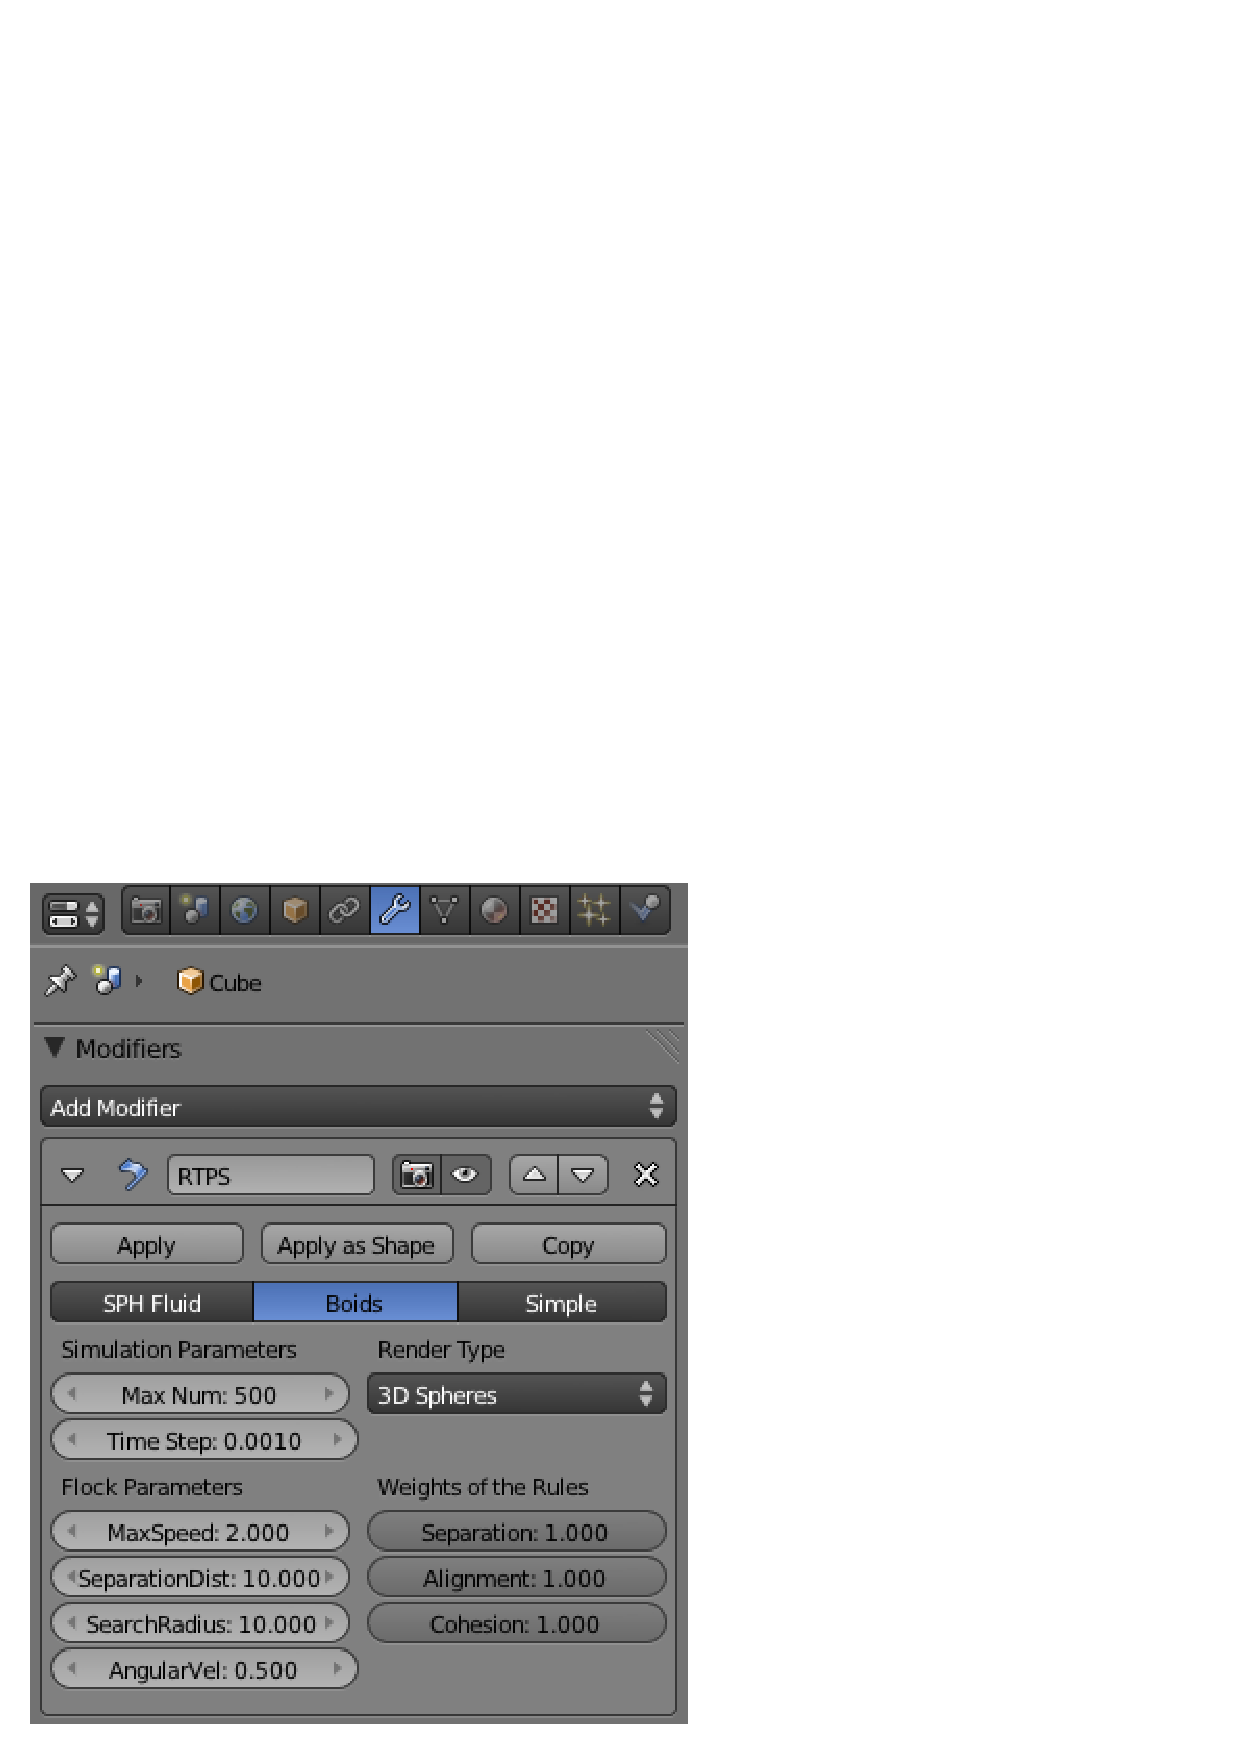
\includegraphics[scale=0.4]{../figures/modifier.pdf}
	%\caption{The RTPS modifier in the Boids system}
	\end{center}
	\end{figure}
\end{frame}

\begin{frame}{Emitting particles to the system}

	\pause
	\begin{columns}
	
	\begin{column}{5cm}
	\begin{table}[htdp]
	%\caption{Properties available in the RTPS modifer}
	\begin{center}
	\begin{tabular}{|p{1.5cm}|p{3cm}|}
	\hline 
	\textbf{Property} & \textbf{Description} \\\hline 
	\texttt{num} 	& num particles are emitted and num is set back to 0	\\\hline 
	\texttt{hose}	& used to active the hose	\\\hline
	\texttt{speed}	& initial velocity of the particles emitted from the hose	\\\hline
	\texttt{radius}	& width of the hose	\\
	\hline 
	\end{tabular}
	\end{center}
	\end{table}
	\end{column}
	
	\begin{column}{5cm}
	\begin{figure}[htbp]
	\begin{center}
	\includegraphics[scale=0.45]{../figures/logic_properties.pdf}
	\end{center}
	\caption{Blender Properties}
	\label{logicEditor}
	\end{figure}
	\end{column}
	
	\end{columns}
\end{frame}


%--------------------------------------------
% results
%--------------------------------------------
\section{Results}

%--------------------------------------------
% timings
%--------------------------------------------
\subsection{Benchmarks}

% RTPS vs RTPS
\begin{frame}{RTPS-FLOCK system}
	\begin{figure}[htbp]
	\begin{center}
	\includegraphics[scale=0.5]{../figures/RTPSvsRTPS.pdf}
	%\caption{Timings of RTPS-FLOCK system}
	\end{center}
	\end{figure}

\end{frame}

% RTPS Blender vs Blender
\begin{frame}{RTPS Blender vs Blender}
	\begin{figure}[htbp]
	\begin{center}
	\includegraphics[scale=0.50]{../figures/benchmarks.pdf}
	%\caption{Timings of RTPS modifier and Blender Boids system}
	\label{plot}
	\end{center}
	\end{figure}
\end{frame}

% speedup
\begin{frame}{Speedup} 
	\begin{figure}[htbp]
	\begin{center}
	\includegraphics[scale=0.50]{../figures/speedup.pdf}
	%\caption{Speedup of the FLOCK system of the RTPS library over the Blender Boids system}
	\label{speedup}
	\end{center}
	\end{figure}
\end{frame}

% RTPS kernels
\begin{frame}{RTPS kernels}
	\begin{figure}[htbp]
	\begin{center}
	\includegraphics[scale=0.50]{../figures/kernelsPlot.pdf}
	%\caption{Timings for the kernels executed by the FLOCK system of RTPS}
	\label{kernelBench}
	\end{center}
	\end{figure}
\end{frame}


%--------------------------------------------
% demos
%--------------------------------------------
\subsection{Demos}

% Symmetry
\begin{frame}{Symmetry Demo}
	\begin{figure}[htbp]
	\begin{center}
	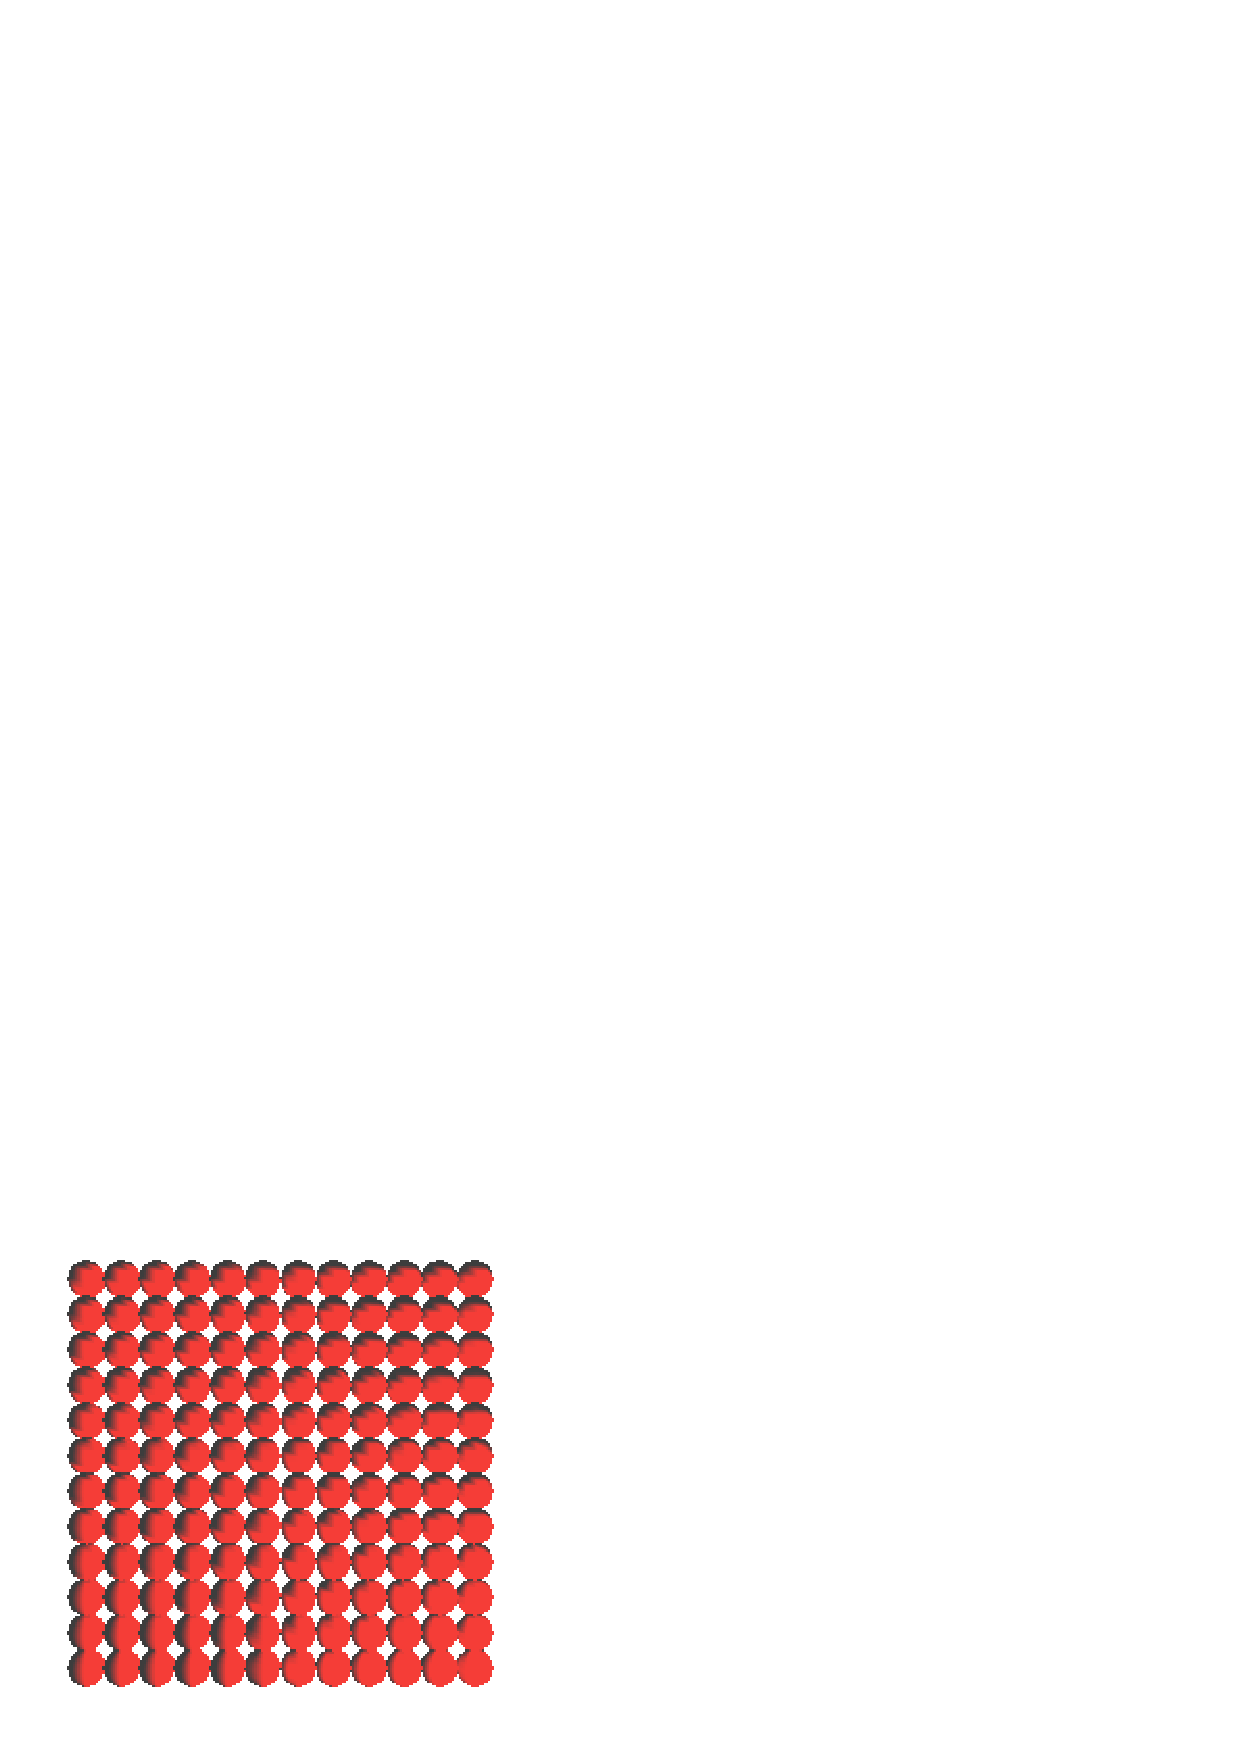
\includegraphics[scale=0.35]{../figures/align.pdf}
	\caption{Initial state of the boids}
	\label{alignRule}
	\end{center}
	\end{figure}
\end{frame}

\begin{frame}{Symmetry Demo: Separation}
	\begin{center}
  		\includemovie[poster, text=(Separation Video), repeat]{6cm}{6cm}{../videos/video_separation.mpg}
	\end{center}
\end{frame}

\begin{frame}{Symmetry Demo: Cohesion}
	\begin{center}
  		\includemovie[poster, text=(Cohesion Video), repeat]{6cm}{6cm}{../videos/video_cohesion.mpg}
	\end{center}
\end{frame}

% Goal Demo
\begin{frame}{Bees approaching their hive simulation}
	\begin{center}
  		\includemovie[poster, text=(Goal Video), repeat]{6cm}{6cm}{../videos/video_goal.mpg}
	\end{center}
\end{frame}

% Blender
\begin{frame}{Crowding simulation}
	\begin{center}
  		\includemovie[poster, text=(Crowding Video), repeat]{10cm}{6cm}{../videos/video_crowd.mov}
	\end{center}
\end{frame}

%--------------------------------------------
% conclusion
%--------------------------------------------
\section{Conclusion}
\begin{frame}{Conclusion}
	\begin{itemize}
		\item Using the RTPS library we were able to implement a flocking algorithm in OpenCL.
		\item A custom modifier was developed in Blender to call the RTPS library.
		\item The RTPS modifier able to run a Boids system inside the Blender Game Engine.
		\item The performance of the RTPS modifier outperforms the Boids system of Blender.
	\end{itemize}
\end{frame}

%--------------------------------------------
% future work
%--------------------------------------------
\subsection{Future Work}
\begin{frame}{Future work}
	\begin{itemize}
		\item Expand the list of the implemented rules.
		\item Use Swarm Intelligence or Evolutionary Algorithm to select an optimized set of parameters for the system.
		\item Hybrids systems.
		\item Use Blender objects as emitter objects.
	\end{itemize}
\end{frame}

%--------------------------------------------
%acknowledgments
%--------------------------------------------
\subsection{Acknowledgements}

\begin{frame}{Acknowledgements}
	\begin{table}[htdp]
	\begin{center}
	\begin{tabular}{ccc}
	 & \textbf{Adviser} &\\
	 & Dr. Gordon Erlebacher &\\ 
	& &  \\
	& &  \\ 
	\textbf{Committee} 		&&  \textbf{Special Recognition}\\ 
	Dr. Xiaoqiang Wang 	&&  Ian Johnson\\ 
	Dr. Ming Ye 			&&  Andrew Young\\ 
	 					&&   Evan Bollig \\
	\end{tabular} 
	\end{center}
	\end{table}
\end{frame}

% questions
\begin{frame}
	\begin{center}
	\textbf{Questions?}
	\end{center}
\end{frame}


\end{document}